\section{Question 6 (Theoretial) and 5 (Simulation)-Frequency Response}
In this section, both octave and ngspice were used in order to obtain plots of the phase response and of the magnitude response, using logscale. This approach is very useful hence it provides a much better plot fit and, therefore it provides great visualization for users. The magnitude in debicels is of interest for analysis of sound waves, and the analysis of the phase or angle delay is a very interesting way of study another parameter to compare signal. Frequency range in both analysis was from 0.1 Hz to 1MHz. The plots made were v6(f), vs(f) and vc=(v6(f)-v8(f)).

\subsection{Theoretical Analysis}

To examine the frequency responses, the system of equations in Section 4 is solved in a loop cycle, what allows us to calculate the $V_6$, $V_c$ and $V_s$ for each frequence. For each result of these complex vectors, the values were saved.

\subsubsection{Frequency Response- Magnitude}

To represent the magnitude in dB, the absolute values were converted ($X_{dB}$=20$log_{10}$(X)). The frequencies were put in a logarithmic scale.

The magnitude of $V_s$ does not suffer any alteration with the variation of the frequency of the signal. Since its amplitude is 1, as one can observe in the graphics shown at the end of the section, the plot shows a constant horizontal line, with the value zero (0=$log_{10}$(1)).

On the contrary, as the frequency is increasing, the magnitudes of $V_6$ and $V_c$ decrease. The value of $V_c$ changes as it is expected in a RC circuit. This is due to the impedance of the capacitor (Z=-j/wC).

\subsubsection{Frequency Response- Phase}


The angles of the values saved were transformed from radians to degrees. The phase in $V_s$ is 0, therefore we do not have to do any further calculations. The phase of each voltage corresponds to the exact angles. In the plot shown below, the frequencies were also  put in the logarithmic scale. As the frequency increases the phase tend to negative values, which varies as it is expected.


\subsection{Simulation Analysis}
In this part of the assignment, an AC (Small Signal Analysis was conducted, in order to match the goal aforementioned. This type of analysis allows to study the frequency response of the circuit. In other words, there is no frequency variation over time, the so called steady-state analysis.

\subsection{Comparison}
After comparing the graphics showed below, it is clear to admit that the results in ngspice and octave match. Any minor difference may be explained by aproximation errors.

\subsubsection{Frequency Response- Magnitude}


\begin{figure}[ht] \centering
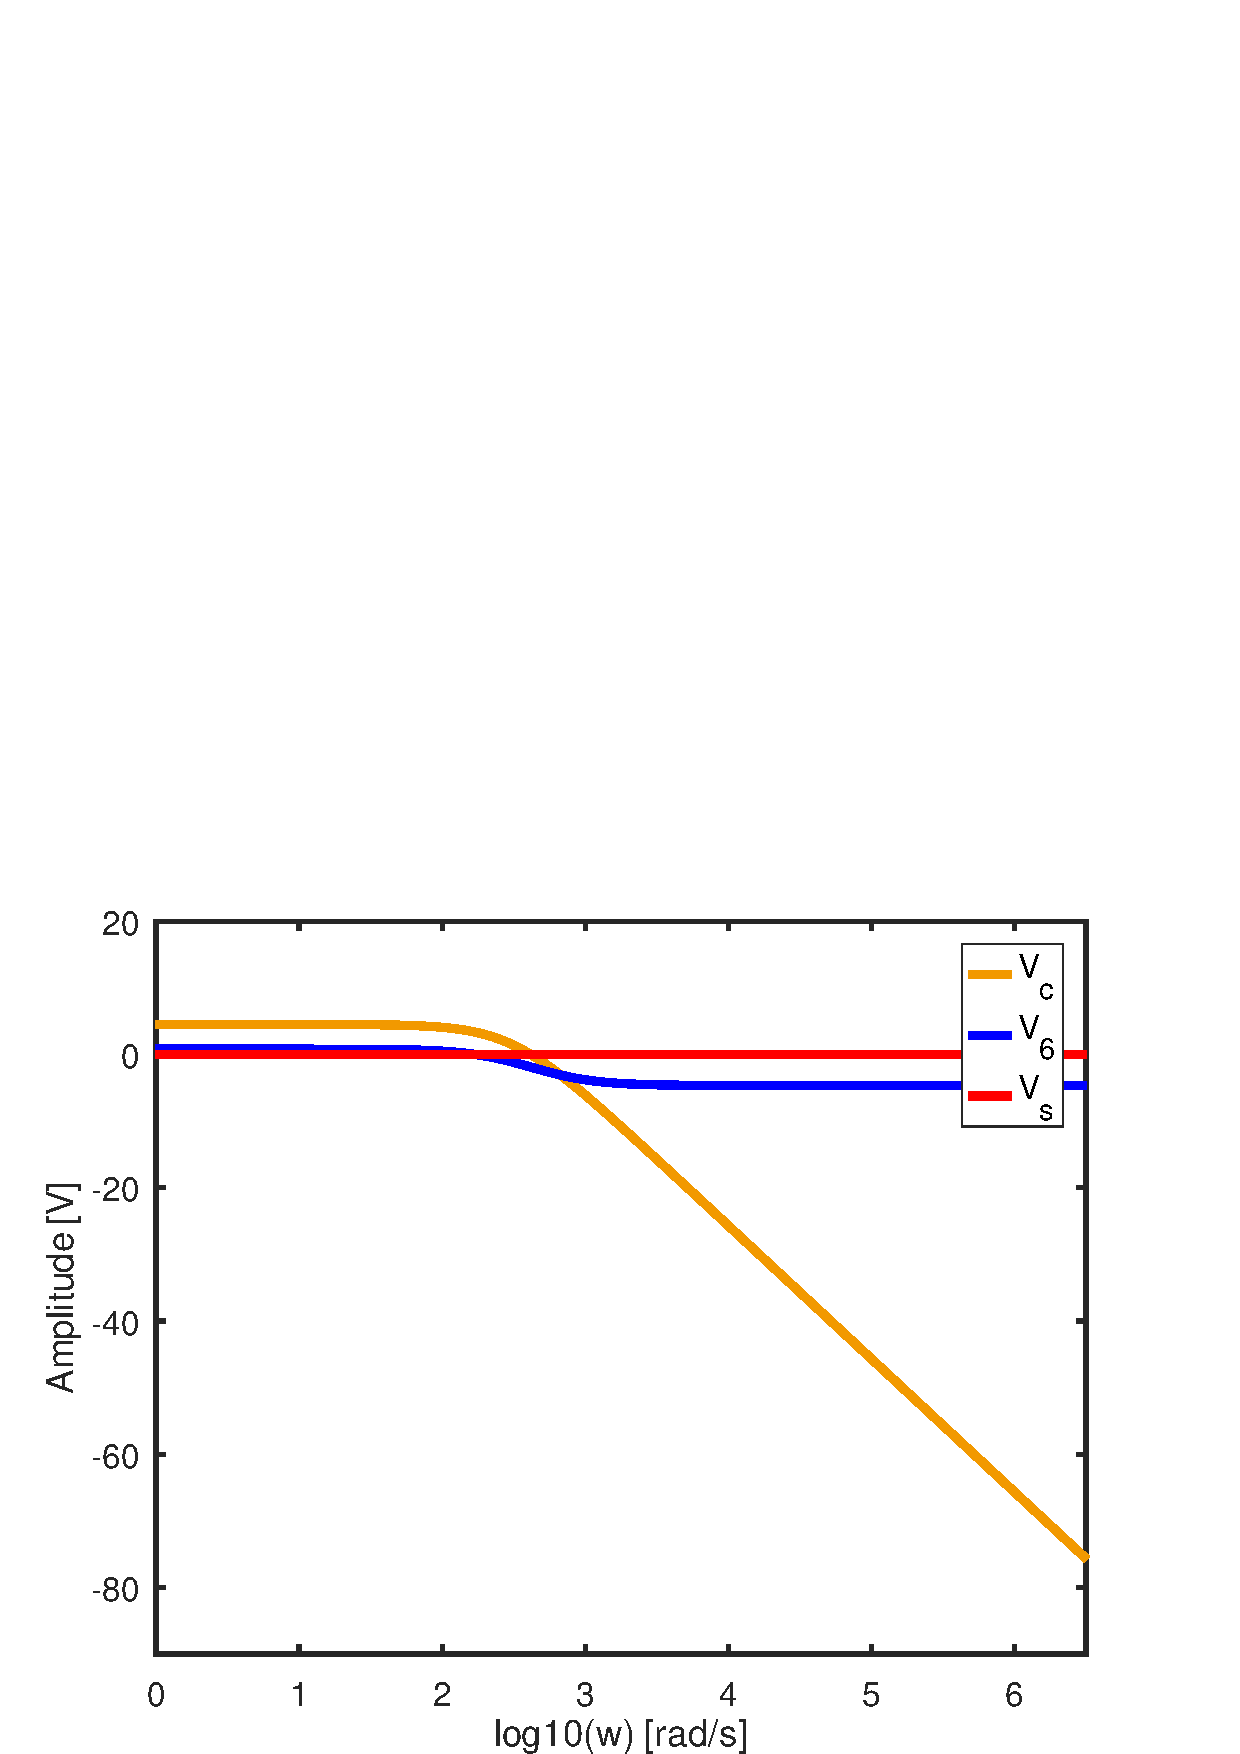
\includegraphics[width=0.9\linewidth]{part6_amp.pdf}
\caption{Circuit analysed.}
\label{RC Circuit.}
\end{figure}


\begin{figure}[ht] \centering
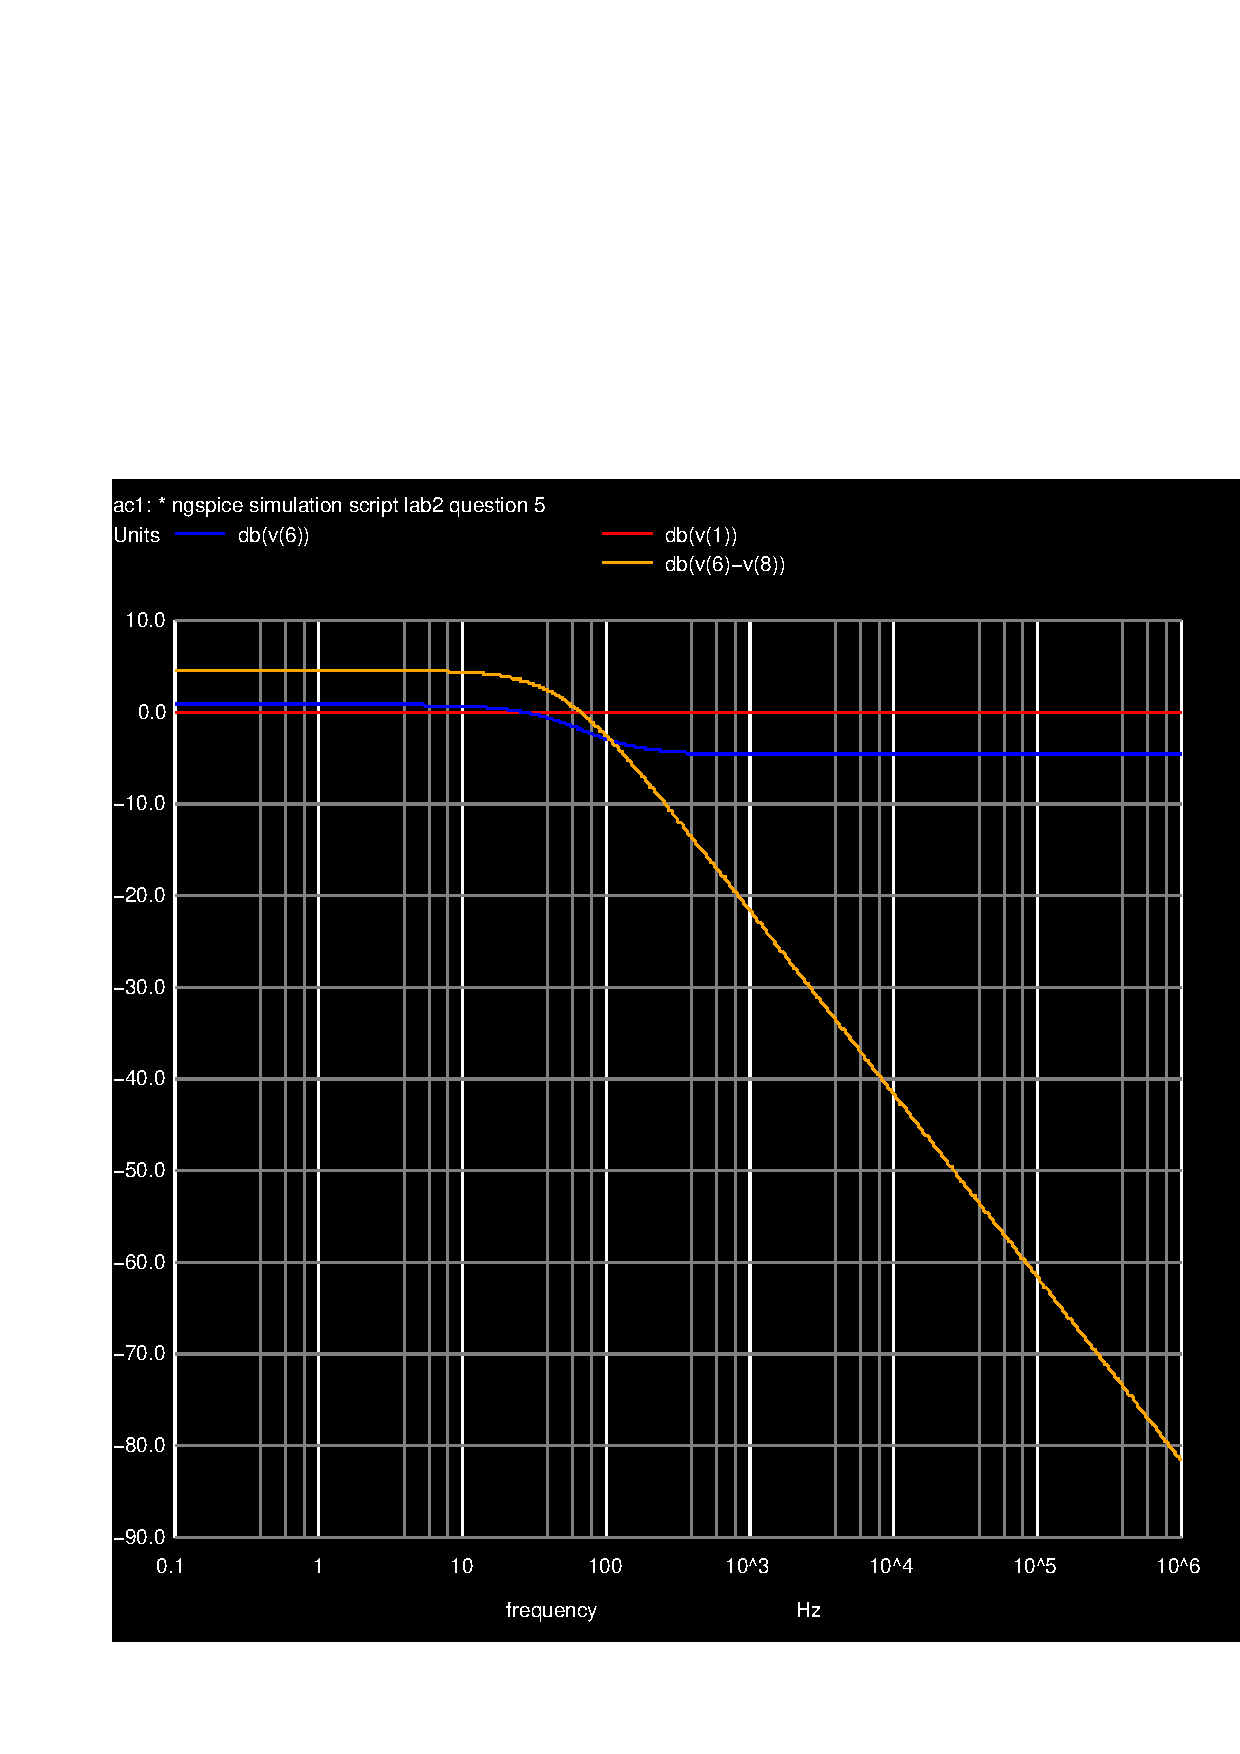
\includegraphics[width=0.9\linewidth]{sim5_db.pdf}
\caption{Magnitude Response (in decibels)}
\label{fig:sim5_db}
\end{figure}

\subsubsection{Frequency Response- Phase}

\begin{figure}[ht] \centering
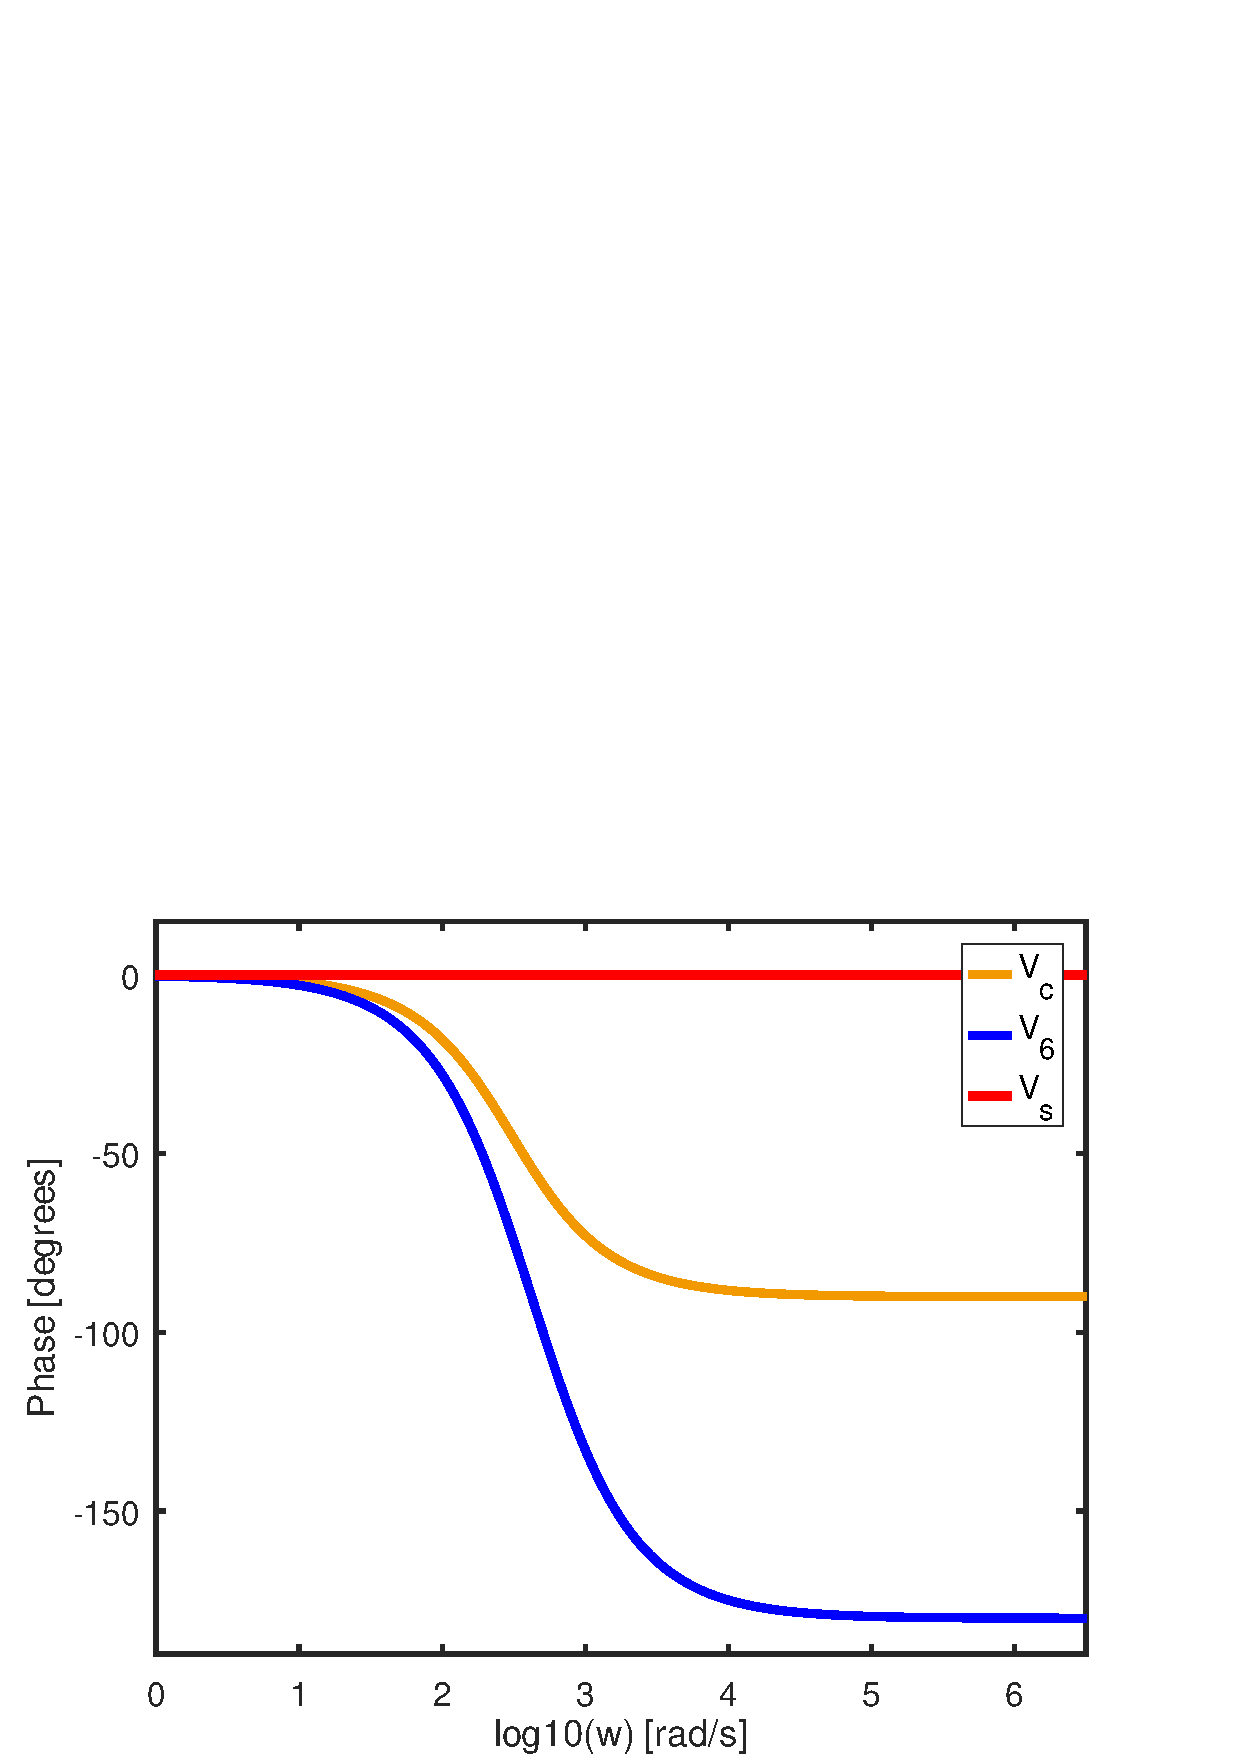
\includegraphics[width=0.9\linewidth]{part6_ang.pdf}
\caption{Circuit analysed.}
\label{RC Circuit.}
\end{figure}

\begin{figure}[ht] \centering
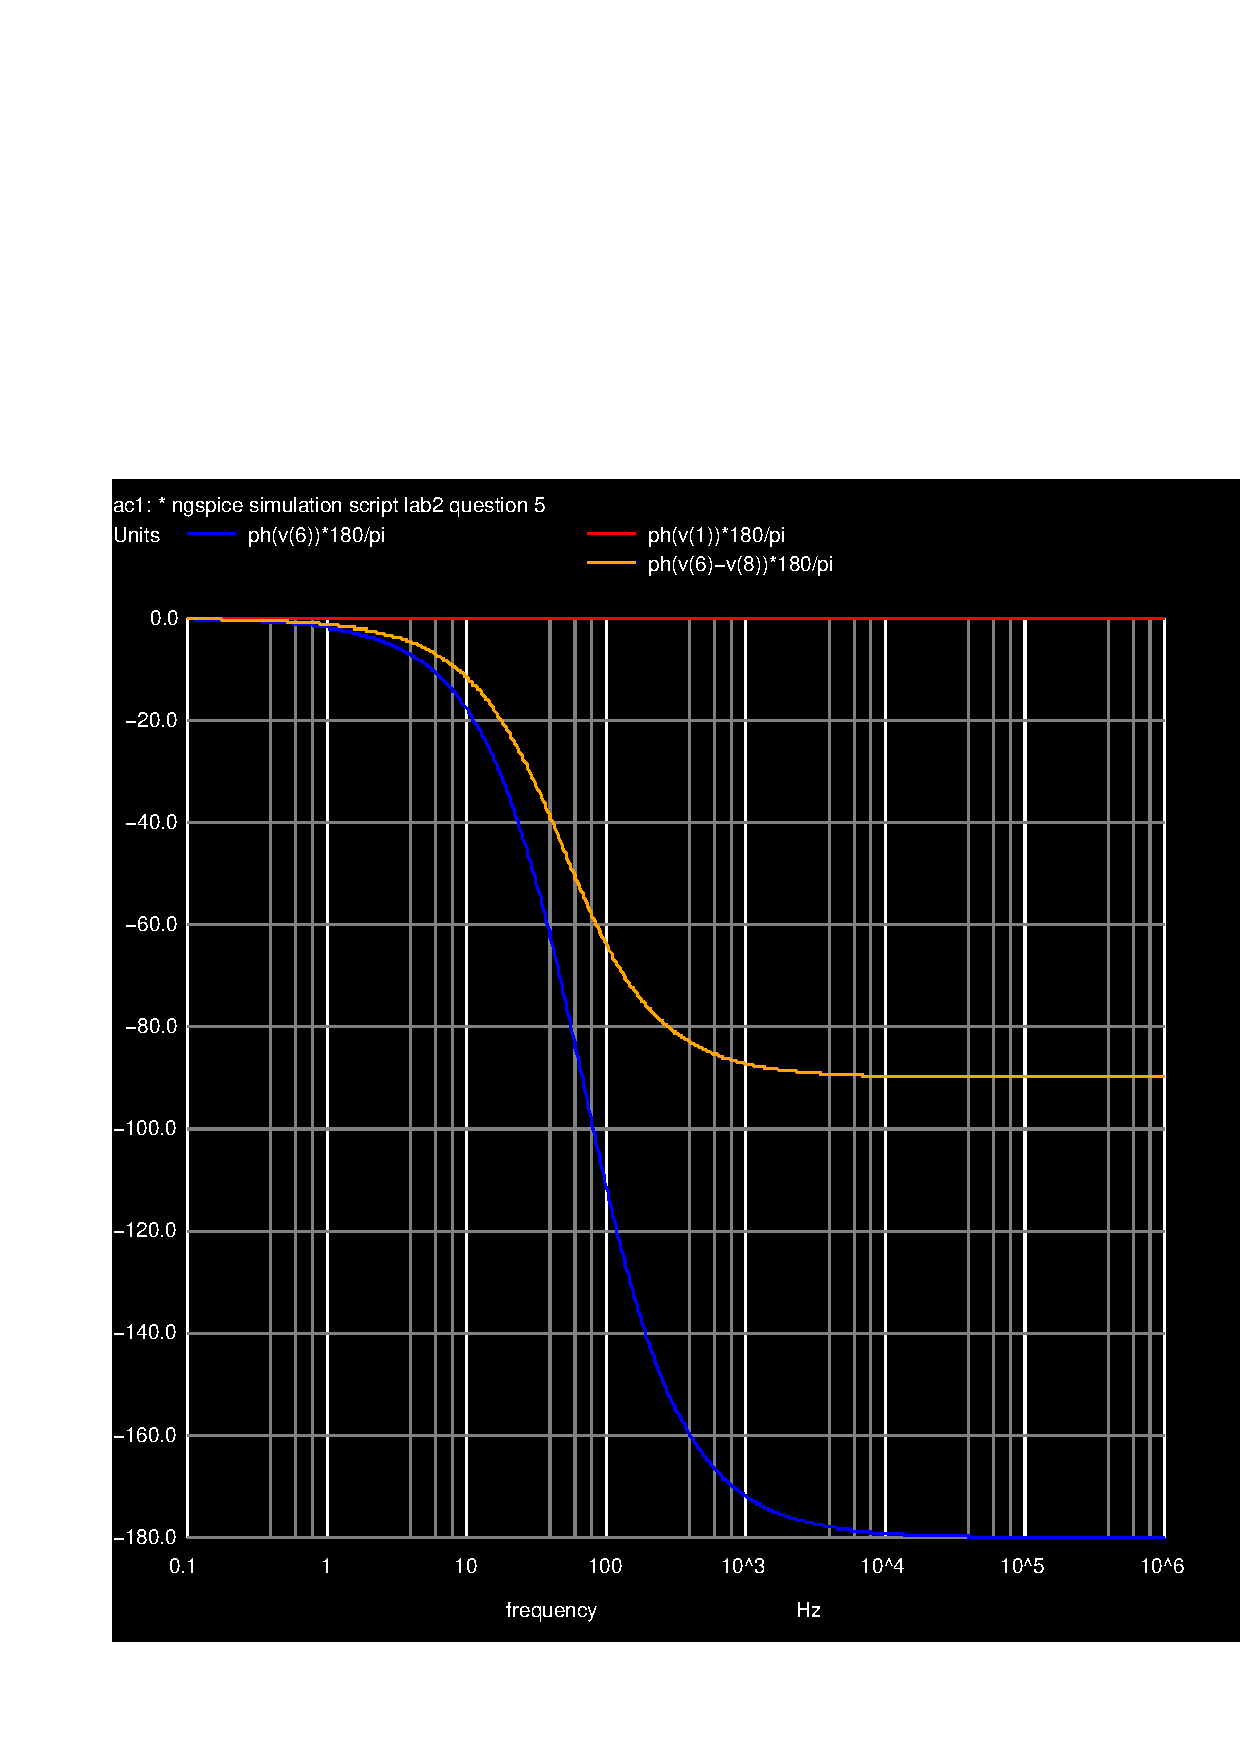
\includegraphics[width=0.9\linewidth]{sim5_ph.pdf}
\caption{Phase Response (in degrees)}
\label{fig:sim5_ph}
\end{figure}
















